\documentclass[twoside]{book}

% Packages required by doxygen
\usepackage{fixltx2e}
\usepackage{calc}
\usepackage{doxygen}
\usepackage[export]{adjustbox} % also loads graphicx
\usepackage{graphicx}
\usepackage[utf8]{inputenc}
\usepackage{makeidx}
\usepackage{multicol}
\usepackage{multirow}
\PassOptionsToPackage{warn}{textcomp}
\usepackage{textcomp}
\usepackage[nointegrals]{wasysym}
\usepackage[table]{xcolor}

% Font selection
\usepackage[T1]{fontenc}
\usepackage[scaled=.90]{helvet}
\usepackage{courier}
\usepackage{amssymb}
\usepackage{sectsty}
\renewcommand{\familydefault}{\sfdefault}
\allsectionsfont{%
  \fontseries{bc}\selectfont%
  \color{darkgray}%
}
\renewcommand{\DoxyLabelFont}{%
  \fontseries{bc}\selectfont%
  \color{darkgray}%
}
\newcommand{\+}{\discretionary{\mbox{\scriptsize$\hookleftarrow$}}{}{}}

% Page & text layout
\usepackage{geometry}
\geometry{%
  a4paper,%
  top=2.5cm,%
  bottom=2.5cm,%
  left=2.5cm,%
  right=2.5cm%
}
\tolerance=750
\hfuzz=15pt
\hbadness=750
\setlength{\emergencystretch}{15pt}
\setlength{\parindent}{0cm}
\setlength{\parskip}{3ex plus 2ex minus 2ex}
\makeatletter
\renewcommand{\paragraph}{%
  \@startsection{paragraph}{4}{0ex}{-1.0ex}{1.0ex}{%
    \normalfont\normalsize\bfseries\SS@parafont%
  }%
}
\renewcommand{\subparagraph}{%
  \@startsection{subparagraph}{5}{0ex}{-1.0ex}{1.0ex}{%
    \normalfont\normalsize\bfseries\SS@subparafont%
  }%
}
\makeatother

% Headers & footers
\usepackage{fancyhdr}
\pagestyle{fancyplain}
\fancyhead[LE]{\fancyplain{}{\bfseries\thepage}}
\fancyhead[CE]{\fancyplain{}{}}
\fancyhead[RE]{\fancyplain{}{\bfseries\leftmark}}
\fancyhead[LO]{\fancyplain{}{\bfseries\rightmark}}
\fancyhead[CO]{\fancyplain{}{}}
\fancyhead[RO]{\fancyplain{}{\bfseries\thepage}}
\fancyfoot[LE]{\fancyplain{}{}}
\fancyfoot[CE]{\fancyplain{}{}}
\fancyfoot[RE]{\fancyplain{}{\bfseries\scriptsize Generated by Doxygen }}
\fancyfoot[LO]{\fancyplain{}{\bfseries\scriptsize Generated by Doxygen }}
\fancyfoot[CO]{\fancyplain{}{}}
\fancyfoot[RO]{\fancyplain{}{}}
\renewcommand{\footrulewidth}{0.4pt}
\renewcommand{\chaptermark}[1]{%
  \markboth{#1}{}%
}
\renewcommand{\sectionmark}[1]{%
  \markright{\thesection\ #1}%
}

% Indices & bibliography
\usepackage{natbib}
\usepackage[titles]{tocloft}
\setcounter{tocdepth}{3}
\setcounter{secnumdepth}{5}
\makeindex

% Hyperlinks (required, but should be loaded last)
\usepackage{ifpdf}
\ifpdf
  \usepackage[pdftex,pagebackref=true]{hyperref}
\else
  \usepackage[ps2pdf,pagebackref=true]{hyperref}
\fi
\hypersetup{%
  colorlinks=true,%
  linkcolor=blue,%
  citecolor=blue,%
  unicode%
}

% Custom commands
\newcommand{\clearemptydoublepage}{%
  \newpage{\pagestyle{empty}\cleardoublepage}%
}

\usepackage{caption}
\captionsetup{labelsep=space,justification=centering,font={bf},singlelinecheck=off,skip=4pt,position=top}

%===== C O N T E N T S =====

\begin{document}

% Titlepage & ToC
\hypersetup{pageanchor=false,
             bookmarksnumbered=true,
             pdfencoding=unicode
            }
\pagenumbering{roman}
\begin{titlepage}
\vspace*{7cm}
\begin{center}%
{\Large My Project }\\
\vspace*{1cm}
{\large Generated by Doxygen 1.8.11}\\
\end{center}
\end{titlepage}
\clearemptydoublepage
\tableofcontents
\clearemptydoublepage
\pagenumbering{arabic}
\hypersetup{pageanchor=true}

%--- Begin generated contents ---
\chapter{Hierarchical Index}
\section{Class Hierarchy}
This inheritance list is sorted roughly, but not completely, alphabetically\+:\begin{DoxyCompactList}
\item \contentsline{section}{Creature}{\pageref{class_creature}}{}
\begin{DoxyCompactList}
\item \contentsline{section}{Animal}{\pageref{class_animal}}{}
\begin{DoxyCompactList}
\item \contentsline{section}{Centaur}{\pageref{class_centaur}}{}
\item \contentsline{section}{Harpy}{\pageref{class_harpy}}{}
\item \contentsline{section}{Lamia}{\pageref{class_lamia}}{}
\end{DoxyCompactList}
\item \contentsline{section}{Plant}{\pageref{class_plant}}{}
\end{DoxyCompactList}
\item \contentsline{section}{Element\+List$<$ Type $>$}{\pageref{class_element_list}}{}
\item \contentsline{section}{Element\+List$<$ Creature $>$}{\pageref{class_element_list}}{}
\item \contentsline{section}{List$<$ Type $>$}{\pageref{class_list}}{}
\item \contentsline{section}{List$<$ Creature $>$}{\pageref{class_list}}{}
\item \contentsline{section}{move\+Direction}{\pageref{structmove_direction}}{}
\item \contentsline{section}{Universe}{\pageref{class_universe}}{}
\begin{DoxyCompactList}
\item \contentsline{section}{Universe\+Using\+List}{\pageref{class_universe_using_list}}{}
\end{DoxyCompactList}
\end{DoxyCompactList}

\chapter{Class Index}
\section{Class List}
Here are the classes, structs, unions and interfaces with brief descriptions\+:\begin{DoxyCompactList}
\item\contentsline{section}{\hyperlink{class_animal}{Animal} }{\pageref{class_animal}}{}
\item\contentsline{section}{\hyperlink{class_centaur}{Centaur} }{\pageref{class_centaur}}{}
\item\contentsline{section}{\hyperlink{class_creature}{Creature} }{\pageref{class_creature}}{}
\item\contentsline{section}{\hyperlink{class_element_list}{Element\+List$<$ Type $>$} }{\pageref{class_element_list}}{}
\item\contentsline{section}{\hyperlink{class_harpy}{Harpy} }{\pageref{class_harpy}}{}
\item\contentsline{section}{\hyperlink{class_lamia}{Lamia} }{\pageref{class_lamia}}{}
\item\contentsline{section}{\hyperlink{class_list}{List$<$ Type $>$} }{\pageref{class_list}}{}
\item\contentsline{section}{\hyperlink{structmove_direction}{move\+Direction} }{\pageref{structmove_direction}}{}
\item\contentsline{section}{\hyperlink{class_plant}{Plant} }{\pageref{class_plant}}{}
\item\contentsline{section}{\hyperlink{class_universe}{Universe} }{\pageref{class_universe}}{}
\item\contentsline{section}{\hyperlink{class_universe_using_list}{Universe\+Using\+List} }{\pageref{class_universe_using_list}}{}
\item\contentsline{section}{\hyperlink{class_universe_using_s_t_l}{Universe\+Using\+S\+TL} }{\pageref{class_universe_using_s_t_l}}{}
\end{DoxyCompactList}

\chapter{Class Documentation}
\hypertarget{class_animal}{}\section{Animal Class Reference}
\label{class_animal}\index{Animal@{Animal}}
Inheritance diagram for Animal\+:\begin{figure}[H]
\begin{center}
\leavevmode
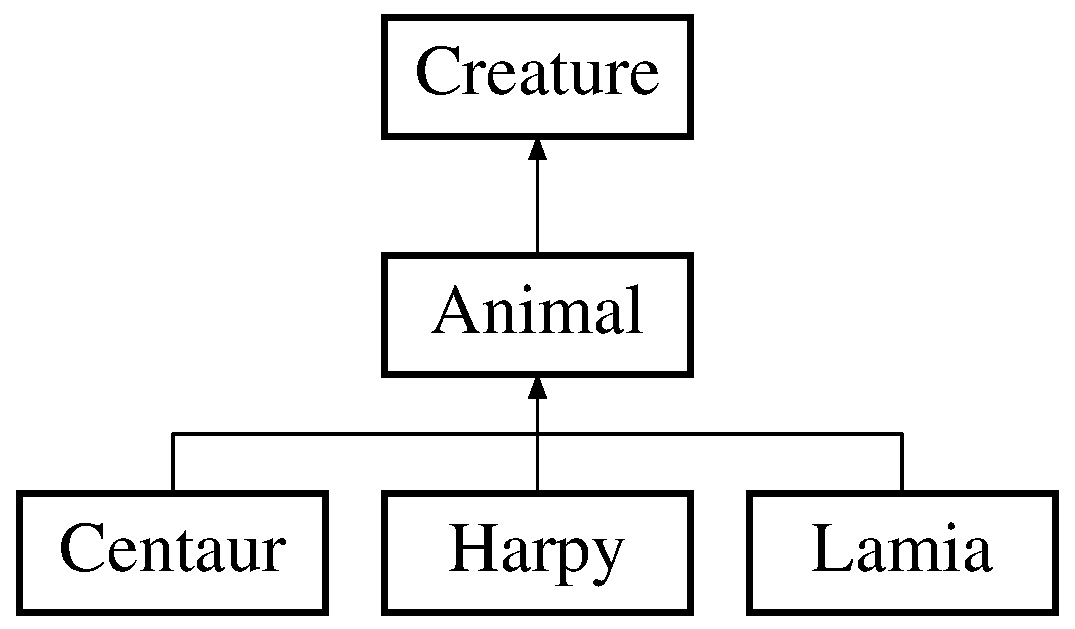
\includegraphics[height=3.000000cm]{class_animal}
\end{center}
\end{figure}
\subsection*{Public Member Functions}
\begin{DoxyCompactItemize}
\item 
\hyperlink{class_animal_a1e726a49ec952443190ac62dad22353c}{Animal} ()
\item 
virtual char {\bfseries draw} ()=0\hypertarget{class_animal_a66c6953f374456d286aa7ae3ab0b80a0}{}\label{class_animal_a66c6953f374456d286aa7ae3ab0b80a0}

\item 
virtual void {\bfseries do\+Action} ()=0\hypertarget{class_animal_a997961a1ecd5c6e0529d8768521b58a9}{}\label{class_animal_a997961a1ecd5c6e0529d8768521b58a9}

\item 
void \hyperlink{class_animal_aee564f22d8d74725c7f718ae5fcf2cd9}{set\+Direction} (int, int)
\item 
\hyperlink{structmove_direction}{move\+Direction} \hyperlink{class_animal_a64d1215d871925e471b94b35ab1f8795}{get\+Direction} ()
\end{DoxyCompactItemize}
\subsection*{Protected Member Functions}
\begin{DoxyCompactItemize}
\item 
virtual void {\bfseries move} ()=0\hypertarget{class_animal_a0b36674071f5144d1e33507b8b90c87d}{}\label{class_animal_a0b36674071f5144d1e33507b8b90c87d}

\end{DoxyCompactItemize}


\subsection{Constructor \& Destructor Documentation}
\index{Animal@{Animal}!Animal@{Animal}}
\index{Animal@{Animal}!Animal@{Animal}}
\subsubsection[{\texorpdfstring{Animal()}{Animal()}}]{\setlength{\rightskip}{0pt plus 5cm}Animal\+::\+Animal (
\begin{DoxyParamCaption}
{}
\end{DoxyParamCaption}
)}\hypertarget{class_animal_a1e726a49ec952443190ac62dad22353c}{}\label{class_animal_a1e726a49ec952443190ac62dad22353c}
Ctor of \hyperlink{class_animal}{Animal} Class do nothing 

\subsection{Member Function Documentation}
\index{Animal@{Animal}!get\+Direction@{get\+Direction}}
\index{get\+Direction@{get\+Direction}!Animal@{Animal}}
\subsubsection[{\texorpdfstring{get\+Direction()}{getDirection()}}]{\setlength{\rightskip}{0pt plus 5cm}{\bf move\+Direction} Animal\+::get\+Direction (
\begin{DoxyParamCaption}
{}
\end{DoxyParamCaption}
)}\hypertarget{class_animal_a64d1215d871925e471b94b35ab1f8795}{}\label{class_animal_a64d1215d871925e471b94b35ab1f8795}
Get the move direction of an \hyperlink{class_animal}{Animal} \begin{DoxyReturn}{Returns}
return the direction attribute of \hyperlink{class_animal}{Animal} 
\end{DoxyReturn}
\index{Animal@{Animal}!set\+Direction@{set\+Direction}}
\index{set\+Direction@{set\+Direction}!Animal@{Animal}}
\subsubsection[{\texorpdfstring{set\+Direction(int, int)}{setDirection(int, int)}}]{\setlength{\rightskip}{0pt plus 5cm}void Animal\+::set\+Direction (
\begin{DoxyParamCaption}
\item[{int}]{x, }
\item[{int}]{y}
\end{DoxyParamCaption}
)}\hypertarget{class_animal_aee564f22d8d74725c7f718ae5fcf2cd9}{}\label{class_animal_aee564f22d8d74725c7f718ae5fcf2cd9}
Set the move direction of an \hyperlink{class_animal}{Animal} 
\begin{DoxyParams}{Parameters}
{\em x} & The horizontal direction with 1 denoting right and -\/1 denothing left \\
\hline
{\em y} & The vertical direction with 1 denoting up and -\/1 denoting down \\
\hline
\end{DoxyParams}


The documentation for this class was generated from the following files\+:\begin{DoxyCompactItemize}
\item 
Animal.\+h\item 
Animal.\+cpp\end{DoxyCompactItemize}

\hypertarget{class_centaur}{}\section{Centaur Class Reference}
\label{class_centaur}\index{Centaur@{Centaur}}
Inheritance diagram for Centaur\+:\begin{figure}[H]
\begin{center}
\leavevmode
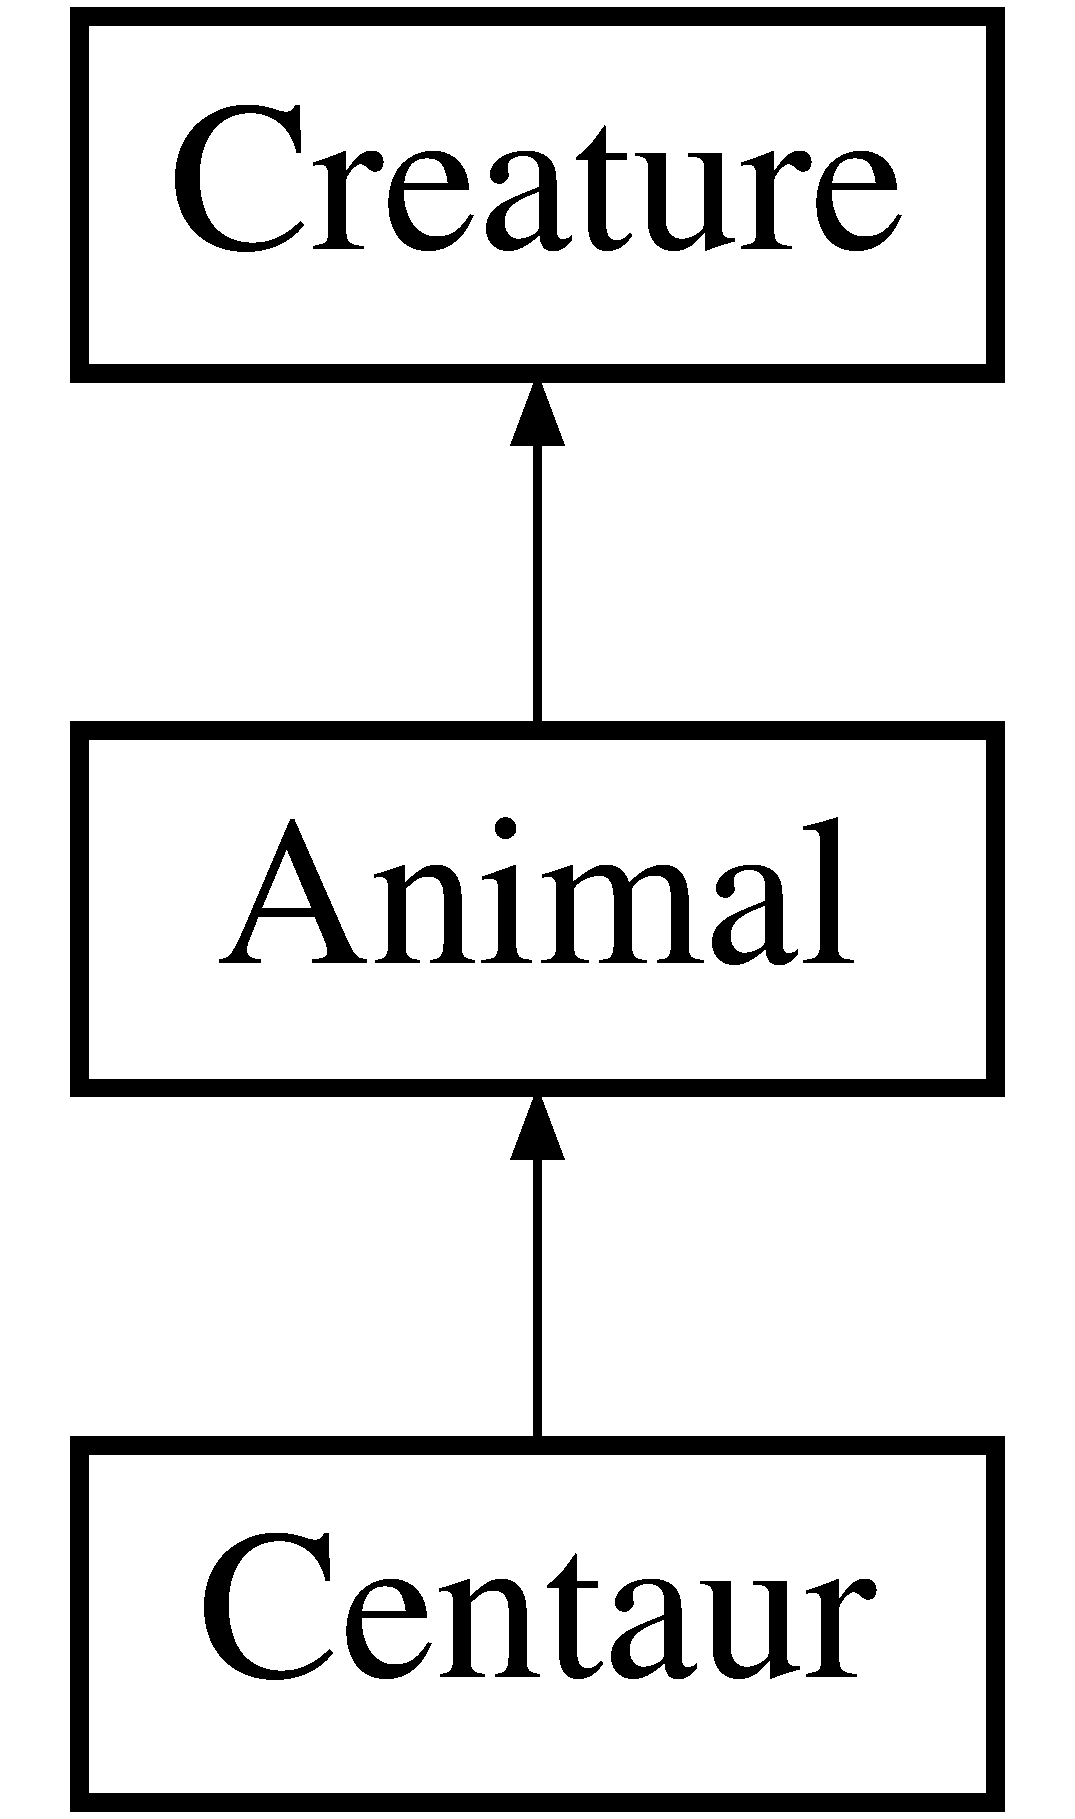
\includegraphics[height=3.000000cm]{class_centaur}
\end{center}
\end{figure}
\subsection*{Public Member Functions}
\begin{DoxyCompactItemize}
\item 
\hyperlink{class_centaur_afc70d85a296f8bb7006525675ee4d92a}{Centaur} (int=0, int=0, int=0, int=0)
\item 
char \hyperlink{class_centaur_a377c0ba95b6599ce868049f551b37b6e}{draw} ()
\item 
void \hyperlink{class_centaur_a548d9ff34d62d1ba596a6dbdd3199216}{do\+Action} ()
\end{DoxyCompactItemize}
\subsection*{Protected Member Functions}
\begin{DoxyCompactItemize}
\item 
void \hyperlink{class_centaur_a3e69089861f1d984eb7528952c3c1d04}{move} ()
\end{DoxyCompactItemize}


\subsection{Constructor \& Destructor Documentation}
\index{Centaur@{Centaur}!Centaur@{Centaur}}
\index{Centaur@{Centaur}!Centaur@{Centaur}}
\subsubsection[{\texorpdfstring{Centaur(int=0, int=0, int=0, int=0)}{Centaur(int=0, int=0, int=0, int=0)}}]{\setlength{\rightskip}{0pt plus 5cm}Centaur\+::\+Centaur (
\begin{DoxyParamCaption}
\item[{int}]{r = {\ttfamily 0}, }
\item[{int}]{c = {\ttfamily 0}, }
\item[{int}]{x = {\ttfamily 0}, }
\item[{int}]{y = {\ttfamily 0}}
\end{DoxyParamCaption}
)}\hypertarget{class_centaur_afc70d85a296f8bb7006525675ee4d92a}{}\label{class_centaur_afc70d85a296f8bb7006525675ee4d92a}
Make \hyperlink{class_centaur}{Centaur} on postion (x,y) 
\begin{DoxyParams}{Parameters}
{\em r} & r is the starting row position of \hyperlink{class_centaur}{Centaur} \\
\hline
{\em c} & c is the starting column position of \hyperlink{class_centaur}{Centaur} \\
\hline
{\em x} & x is hoizontal component of \hyperlink{structmove_direction}{move\+Direction} \\
\hline
{\em y} & y is vertical componen of \hyperlink{structmove_direction}{move\+Direction} \\
\hline
\end{DoxyParams}


\subsection{Member Function Documentation}
\index{Centaur@{Centaur}!do\+Action@{do\+Action}}
\index{do\+Action@{do\+Action}!Centaur@{Centaur}}
\subsubsection[{\texorpdfstring{do\+Action()}{doAction()}}]{\setlength{\rightskip}{0pt plus 5cm}void Centaur\+::do\+Action (
\begin{DoxyParamCaption}
{}
\end{DoxyParamCaption}
)\hspace{0.3cm}{\ttfamily [virtual]}}\hypertarget{class_centaur_a548d9ff34d62d1ba596a6dbdd3199216}{}\label{class_centaur_a548d9ff34d62d1ba596a6dbdd3199216}
Make creature do some kind of action 

Implements \hyperlink{class_animal}{Animal}.

\index{Centaur@{Centaur}!draw@{draw}}
\index{draw@{draw}!Centaur@{Centaur}}
\subsubsection[{\texorpdfstring{draw()}{draw()}}]{\setlength{\rightskip}{0pt plus 5cm}char Centaur\+::draw (
\begin{DoxyParamCaption}
{}
\end{DoxyParamCaption}
)\hspace{0.3cm}{\ttfamily [virtual]}}\hypertarget{class_centaur_a377c0ba95b6599ce868049f551b37b6e}{}\label{class_centaur_a377c0ba95b6599ce868049f551b37b6e}
Draw the \hyperlink{class_centaur}{Centaur} by returning its character symbol \begin{DoxyReturn}{Returns}
Special char denoting \hyperlink{class_centaur}{Centaur} 
\end{DoxyReturn}


Implements \hyperlink{class_animal}{Animal}.

\index{Centaur@{Centaur}!move@{move}}
\index{move@{move}!Centaur@{Centaur}}
\subsubsection[{\texorpdfstring{move()}{move()}}]{\setlength{\rightskip}{0pt plus 5cm}void Centaur\+::move (
\begin{DoxyParamCaption}
{}
\end{DoxyParamCaption}
)\hspace{0.3cm}{\ttfamily [protected]}, {\ttfamily [virtual]}}\hypertarget{class_centaur_a3e69089861f1d984eb7528952c3c1d04}{}\label{class_centaur_a3e69089861f1d984eb7528952c3c1d04}
Move the \hyperlink{class_centaur}{Centaur} one step according to its \hyperlink{structmove_direction}{move\+Direction} 

Implements \hyperlink{class_animal}{Animal}.



The documentation for this class was generated from the following files\+:\begin{DoxyCompactItemize}
\item 
Centaur.\+h\item 
Centaur.\+cpp\end{DoxyCompactItemize}

\hypertarget{class_creature}{}\section{Creature Class Reference}
\label{class_creature}\index{Creature@{Creature}}
Inheritance diagram for Creature\+:\begin{figure}[H]
\begin{center}
\leavevmode
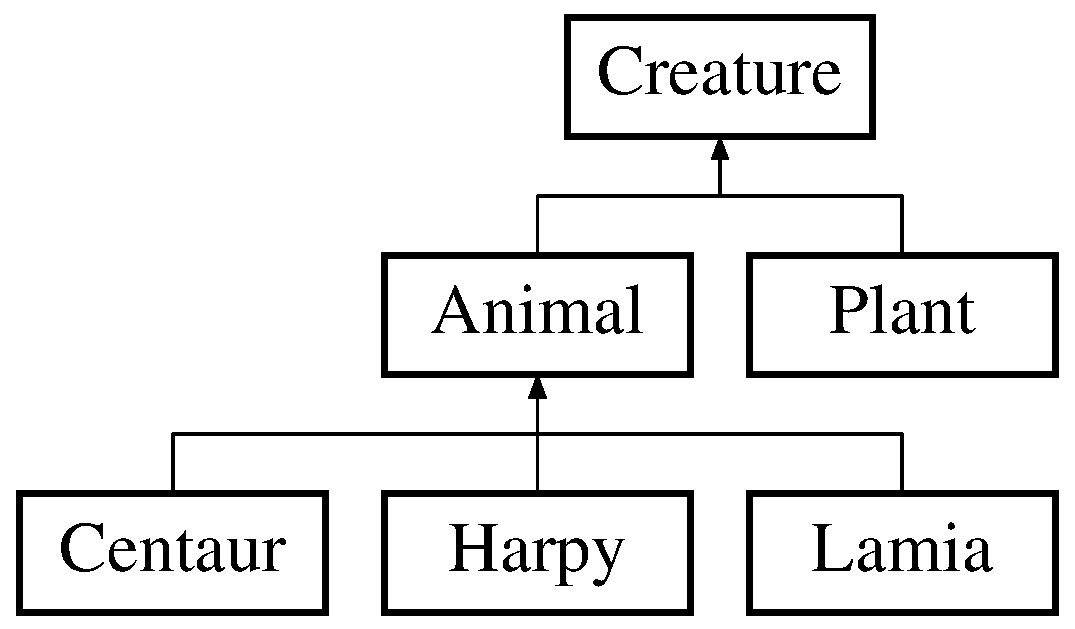
\includegraphics[height=3.000000cm]{class_creature}
\end{center}
\end{figure}
\subsection*{Public Member Functions}
\begin{DoxyCompactItemize}
\item 
virtual char {\bfseries draw} ()=0\hypertarget{class_creature_a5be2a9f038cd7641974462a80a009198}{}\label{class_creature_a5be2a9f038cd7641974462a80a009198}

\item 
virtual void {\bfseries do\+Action} ()=0\hypertarget{class_creature_ae40c732ab8eccea97404b9282fdd1138}{}\label{class_creature_ae40c732ab8eccea97404b9282fdd1138}

\item 
void {\bfseries set\+Row\+Position} (int)\hypertarget{class_creature_a1bc33218a560eff8162a2e795e90251f}{}\label{class_creature_a1bc33218a560eff8162a2e795e90251f}

\item 
void {\bfseries set\+Column\+Position} (int)\hypertarget{class_creature_a4ab0c6b21b0826ed9691583eec078bec}{}\label{class_creature_a4ab0c6b21b0826ed9691583eec078bec}

\item 
void {\bfseries set\+Strength} (int)\hypertarget{class_creature_a032ac31736090da076da0ec1466c27bf}{}\label{class_creature_a032ac31736090da076da0ec1466c27bf}

\item 
int {\bfseries get\+Row\+Position} ()\hypertarget{class_creature_a8062f777315929e10e5d626e95366438}{}\label{class_creature_a8062f777315929e10e5d626e95366438}

\item 
int {\bfseries get\+Column\+Position} ()\hypertarget{class_creature_addfbfaf75df9268fa1288c29c50abcd0}{}\label{class_creature_addfbfaf75df9268fa1288c29c50abcd0}

\item 
int {\bfseries get\+Strength} ()\hypertarget{class_creature_aae311cca00cca409e3e790a96ad14b97}{}\label{class_creature_aae311cca00cca409e3e790a96ad14b97}

\end{DoxyCompactItemize}


The documentation for this class was generated from the following files\+:\begin{DoxyCompactItemize}
\item 
Creature.\+h\item 
Creature.\+cpp\end{DoxyCompactItemize}

\hypertarget{class_element_list}{}\section{Element\+List$<$ Type $>$ Class Template Reference}
\label{class_element_list}\index{Element\+List$<$ Type $>$@{Element\+List$<$ Type $>$}}
\subsection*{Public Member Functions}
\begin{DoxyCompactItemize}
\item 
\hyperlink{class_element_list_a0157b98943770fe3f09bda77d99a8641}{Element\+List} ()
\item 
\hyperlink{class_element_list_a042a80b094d946d3e6526ab8321e32f7}{Element\+List} (Type \&data)
\item 
\hyperlink{class_element_list_adf838c89433130d312b11c7e304b710b}{$\sim$\+Element\+List} ()
\item 
Type \hyperlink{class_element_list_a0f874b08fce53174aa75eedf45682d64}{Value} ()
\item 
\hyperlink{class_element_list}{Element\+List} $\ast$ \hyperlink{class_element_list_a2644dc854591779ec7220fd56e0a16ba}{Next} ()
\item 
\hyperlink{class_element_list}{Element\+List} $\ast$ \hyperlink{class_element_list_a5144ccc57d38ce60ec3d5d82471579f6}{Previous} ()
\item 
void \hyperlink{class_element_list_a55fedd16d90c0b856117e02e837e311e}{Delete\+Single} ()
\item 
void \hyperlink{class_element_list_a7c1472ac483bdef89e6fc5370591b6f7}{Set\+Value} (Type \&data)
\item 
void \hyperlink{class_element_list_af4c19f75c4c93b69f2023420ba477f7d}{Set\+Next} (\hyperlink{class_element_list}{Element\+List} $\ast$P)
\item 
void \hyperlink{class_element_list_a60590a74e879b84d87dc3f32bd9ad801}{Set\+Previous} (\hyperlink{class_element_list}{Element\+List} $\ast$P)
\end{DoxyCompactItemize}


\subsection{Constructor \& Destructor Documentation}
\index{Element\+List@{Element\+List}!Element\+List@{Element\+List}}
\index{Element\+List@{Element\+List}!Element\+List@{Element\+List}}
\subsubsection[{\texorpdfstring{Element\+List()}{ElementList()}}]{\setlength{\rightskip}{0pt plus 5cm}template$<$class Type $>$ {\bf Element\+List}$<$ Type $>$\+::{\bf Element\+List} (
\begin{DoxyParamCaption}
{}
\end{DoxyParamCaption}
)}\hypertarget{class_element_list_a0157b98943770fe3f09bda77d99a8641}{}\label{class_element_list_a0157b98943770fe3f09bda77d99a8641}
ctor of \hyperlink{class_element_list}{Element\+List} \index{Element\+List@{Element\+List}!Element\+List@{Element\+List}}
\index{Element\+List@{Element\+List}!Element\+List@{Element\+List}}
\subsubsection[{\texorpdfstring{Element\+List(\+Type \&data)}{ElementList(Type &data)}}]{\setlength{\rightskip}{0pt plus 5cm}template$<$class Type$>$ {\bf Element\+List}$<$ Type $>$\+::{\bf Element\+List} (
\begin{DoxyParamCaption}
\item[{Type \&}]{data}
\end{DoxyParamCaption}
)}\hypertarget{class_element_list_a042a80b094d946d3e6526ab8321e32f7}{}\label{class_element_list_a042a80b094d946d3e6526ab8321e32f7}
ctor with parameter of \hyperlink{class_element_list}{Element\+List} \index{Element\+List@{Element\+List}!````~Element\+List@{$\sim$\+Element\+List}}
\index{````~Element\+List@{$\sim$\+Element\+List}!Element\+List@{Element\+List}}
\subsubsection[{\texorpdfstring{$\sim$\+Element\+List()}{~ElementList()}}]{\setlength{\rightskip}{0pt plus 5cm}template$<$class Type $>$ {\bf Element\+List}$<$ Type $>$\+::$\sim${\bf Element\+List} (
\begin{DoxyParamCaption}
{}
\end{DoxyParamCaption}
)}\hypertarget{class_element_list_adf838c89433130d312b11c7e304b710b}{}\label{class_element_list_adf838c89433130d312b11c7e304b710b}
dtor of \hyperlink{class_element_list}{Element\+List} 

\subsection{Member Function Documentation}
\index{Element\+List@{Element\+List}!Delete\+Single@{Delete\+Single}}
\index{Delete\+Single@{Delete\+Single}!Element\+List@{Element\+List}}
\subsubsection[{\texorpdfstring{Delete\+Single()}{DeleteSingle()}}]{\setlength{\rightskip}{0pt plus 5cm}template$<$class Type $>$ void {\bf Element\+List}$<$ Type $>$\+::Delete\+Single (
\begin{DoxyParamCaption}
{}
\end{DoxyParamCaption}
)}\hypertarget{class_element_list_a55fedd16d90c0b856117e02e837e311e}{}\label{class_element_list_a55fedd16d90c0b856117e02e837e311e}
Erase an element\+List by switching it with last element\+List of it\textquotesingle{}s \hyperlink{class_list}{List} or erase it if it\textquotesingle{}s single element\+List. \index{Element\+List@{Element\+List}!Next@{Next}}
\index{Next@{Next}!Element\+List@{Element\+List}}
\subsubsection[{\texorpdfstring{Next()}{Next()}}]{\setlength{\rightskip}{0pt plus 5cm}template$<$class Type $>$ {\bf Element\+List}$<$ Type $>$ $\ast$ {\bf Element\+List}$<$ Type $>$\+::Next (
\begin{DoxyParamCaption}
{}
\end{DoxyParamCaption}
)}\hypertarget{class_element_list_a2644dc854591779ec7220fd56e0a16ba}{}\label{class_element_list_a2644dc854591779ec7220fd56e0a16ba}
Get the pointer of Next Elemnt \index{Element\+List@{Element\+List}!Previous@{Previous}}
\index{Previous@{Previous}!Element\+List@{Element\+List}}
\subsubsection[{\texorpdfstring{Previous()}{Previous()}}]{\setlength{\rightskip}{0pt plus 5cm}template$<$class Type $>$ {\bf Element\+List}$<$ Type $>$ $\ast$ {\bf Element\+List}$<$ Type $>$\+::Previous (
\begin{DoxyParamCaption}
{}
\end{DoxyParamCaption}
)}\hypertarget{class_element_list_a5144ccc57d38ce60ec3d5d82471579f6}{}\label{class_element_list_a5144ccc57d38ce60ec3d5d82471579f6}
Get the pointer of Previous Elemnt \index{Element\+List@{Element\+List}!Set\+Next@{Set\+Next}}
\index{Set\+Next@{Set\+Next}!Element\+List@{Element\+List}}
\subsubsection[{\texorpdfstring{Set\+Next(\+Element\+List $\ast$\+P)}{SetNext(ElementList *P)}}]{\setlength{\rightskip}{0pt plus 5cm}template$<$class Type $>$ void {\bf Element\+List}$<$ Type $>$\+::Set\+Next (
\begin{DoxyParamCaption}
\item[{{\bf Element\+List}$<$ Type $>$ $\ast$}]{P}
\end{DoxyParamCaption}
)}\hypertarget{class_element_list_af4c19f75c4c93b69f2023420ba477f7d}{}\label{class_element_list_af4c19f75c4c93b69f2023420ba477f7d}
Set the pointer of Next Elemnt 
\begin{DoxyParams}{Parameters}
{\em P} & \\
\hline
\end{DoxyParams}
\index{Element\+List@{Element\+List}!Set\+Previous@{Set\+Previous}}
\index{Set\+Previous@{Set\+Previous}!Element\+List@{Element\+List}}
\subsubsection[{\texorpdfstring{Set\+Previous(\+Element\+List $\ast$\+P)}{SetPrevious(ElementList *P)}}]{\setlength{\rightskip}{0pt plus 5cm}template$<$class Type $>$ void {\bf Element\+List}$<$ Type $>$\+::Set\+Previous (
\begin{DoxyParamCaption}
\item[{{\bf Element\+List}$<$ Type $>$ $\ast$}]{P}
\end{DoxyParamCaption}
)}\hypertarget{class_element_list_a60590a74e879b84d87dc3f32bd9ad801}{}\label{class_element_list_a60590a74e879b84d87dc3f32bd9ad801}
Set the pointer of Previous Elemnt 
\begin{DoxyParams}{Parameters}
{\em P} & \\
\hline
\end{DoxyParams}
\index{Element\+List@{Element\+List}!Set\+Value@{Set\+Value}}
\index{Set\+Value@{Set\+Value}!Element\+List@{Element\+List}}
\subsubsection[{\texorpdfstring{Set\+Value(\+Type \&data)}{SetValue(Type &data)}}]{\setlength{\rightskip}{0pt plus 5cm}template$<$class Type$>$ void {\bf Element\+List}$<$ Type $>$\+::Set\+Value (
\begin{DoxyParamCaption}
\item[{Type \&}]{data}
\end{DoxyParamCaption}
)}\hypertarget{class_element_list_a7c1472ac483bdef89e6fc5370591b6f7}{}\label{class_element_list_a7c1472ac483bdef89e6fc5370591b6f7}
Set the Value of this Element 
\begin{DoxyParams}{Parameters}
{\em data} & \\
\hline
\end{DoxyParams}
\index{Element\+List@{Element\+List}!Value@{Value}}
\index{Value@{Value}!Element\+List@{Element\+List}}
\subsubsection[{\texorpdfstring{Value()}{Value()}}]{\setlength{\rightskip}{0pt plus 5cm}template$<$class Type $>$ Type {\bf Element\+List}$<$ Type $>$\+::Value (
\begin{DoxyParamCaption}
{}
\end{DoxyParamCaption}
)}\hypertarget{class_element_list_a0f874b08fce53174aa75eedf45682d64}{}\label{class_element_list_a0f874b08fce53174aa75eedf45682d64}
Get the value of this elemnt 

The documentation for this class was generated from the following files\+:\begin{DoxyCompactItemize}
\item 
element\+List.\+h\item 
element\+List.\+cpp\end{DoxyCompactItemize}

\hypertarget{class_harpy}{}\section{Harpy Class Reference}
\label{class_harpy}\index{Harpy@{Harpy}}
Inheritance diagram for Harpy\+:\begin{figure}[H]
\begin{center}
\leavevmode
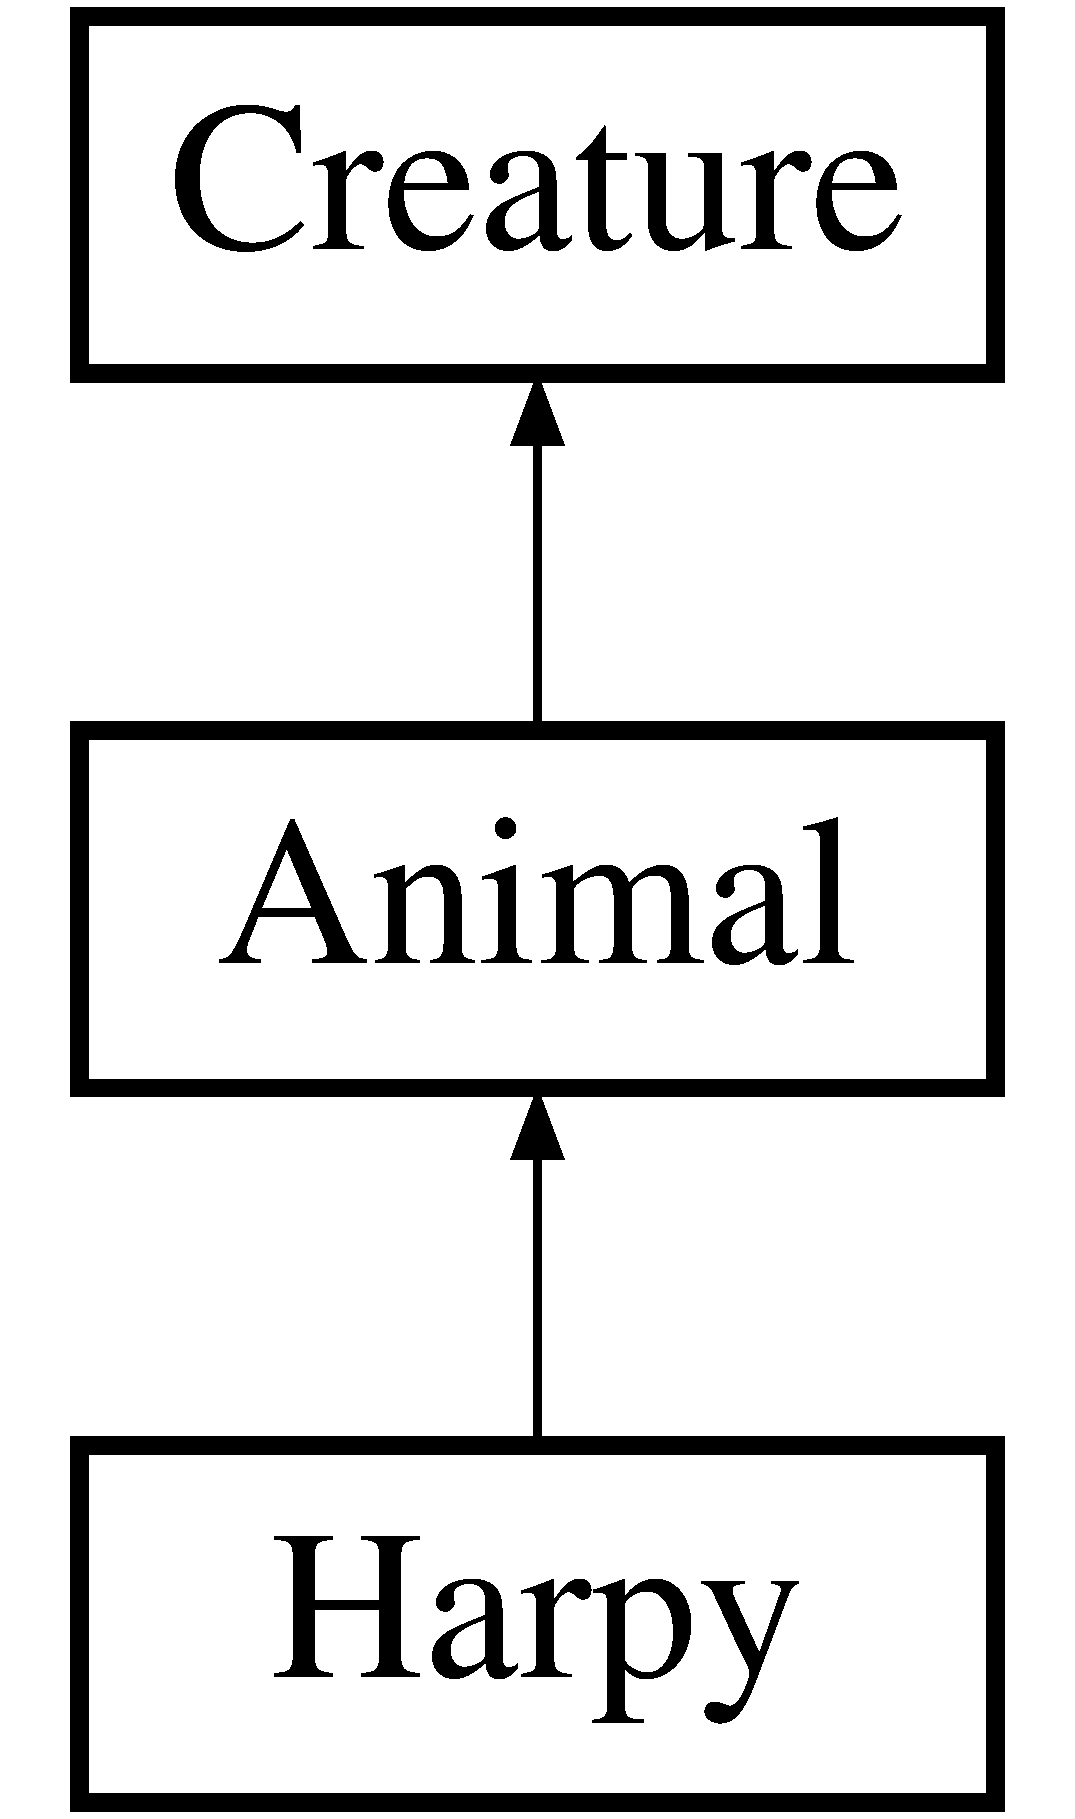
\includegraphics[height=3.000000cm]{class_harpy}
\end{center}
\end{figure}
\subsection*{Public Member Functions}
\begin{DoxyCompactItemize}
\item 
\hyperlink{class_harpy_abf2c43ecb0e635d9b3027e9f1b246067}{Harpy} (int=0, int=0, int=0, int=0)
\item 
void \hyperlink{class_harpy_ab296058454b33ba304b2f6533bcd1994}{do\+Action} ()
\item 
char \hyperlink{class_harpy_aff50872bc2e137a69e4eacc45a739d95}{draw} ()
\end{DoxyCompactItemize}
\subsection*{Protected Member Functions}
\begin{DoxyCompactItemize}
\item 
void \hyperlink{class_harpy_a0a4f8328e78902b76fba8eecf5e0c99e}{move} ()
\end{DoxyCompactItemize}


\subsection{Constructor \& Destructor Documentation}
\index{Harpy@{Harpy}!Harpy@{Harpy}}
\index{Harpy@{Harpy}!Harpy@{Harpy}}
\subsubsection[{\texorpdfstring{Harpy(int=0, int=0, int=0, int=0)}{Harpy(int=0, int=0, int=0, int=0)}}]{\setlength{\rightskip}{0pt plus 5cm}Harpy\+::\+Harpy (
\begin{DoxyParamCaption}
\item[{int}]{r = {\ttfamily 0}, }
\item[{int}]{c = {\ttfamily 0}, }
\item[{int}]{x = {\ttfamily 0}, }
\item[{int}]{y = {\ttfamily 0}}
\end{DoxyParamCaption}
)}\hypertarget{class_harpy_abf2c43ecb0e635d9b3027e9f1b246067}{}\label{class_harpy_abf2c43ecb0e635d9b3027e9f1b246067}
Make \hyperlink{class_harpy}{Harpy} on postion (x,y) 
\begin{DoxyParams}{Parameters}
{\em r} & r is the starting row position of \hyperlink{class_harpy}{Harpy} \\
\hline
{\em c} & c is the starting column position of \hyperlink{class_harpy}{Harpy} \\
\hline
{\em x} & x is hoizontal component of \hyperlink{structmove_direction}{move\+Direction} \\
\hline
{\em y} & y is vertical componen of \hyperlink{structmove_direction}{move\+Direction} \\
\hline
\end{DoxyParams}


\subsection{Member Function Documentation}
\index{Harpy@{Harpy}!do\+Action@{do\+Action}}
\index{do\+Action@{do\+Action}!Harpy@{Harpy}}
\subsubsection[{\texorpdfstring{do\+Action()}{doAction()}}]{\setlength{\rightskip}{0pt plus 5cm}void Harpy\+::do\+Action (
\begin{DoxyParamCaption}
{}
\end{DoxyParamCaption}
)\hspace{0.3cm}{\ttfamily [virtual]}}\hypertarget{class_harpy_ab296058454b33ba304b2f6533bcd1994}{}\label{class_harpy_ab296058454b33ba304b2f6533bcd1994}
Make creature do some kind of action 

Implements \hyperlink{class_animal}{Animal}.

\index{Harpy@{Harpy}!draw@{draw}}
\index{draw@{draw}!Harpy@{Harpy}}
\subsubsection[{\texorpdfstring{draw()}{draw()}}]{\setlength{\rightskip}{0pt plus 5cm}char Harpy\+::draw (
\begin{DoxyParamCaption}
{}
\end{DoxyParamCaption}
)\hspace{0.3cm}{\ttfamily [virtual]}}\hypertarget{class_harpy_aff50872bc2e137a69e4eacc45a739d95}{}\label{class_harpy_aff50872bc2e137a69e4eacc45a739d95}
Draw the \hyperlink{class_harpy}{Harpy} by returning its character symbol \begin{DoxyReturn}{Returns}
Special char denoting \hyperlink{class_harpy}{Harpy} 
\end{DoxyReturn}


Implements \hyperlink{class_animal}{Animal}.

\index{Harpy@{Harpy}!move@{move}}
\index{move@{move}!Harpy@{Harpy}}
\subsubsection[{\texorpdfstring{move()}{move()}}]{\setlength{\rightskip}{0pt plus 5cm}void Harpy\+::move (
\begin{DoxyParamCaption}
{}
\end{DoxyParamCaption}
)\hspace{0.3cm}{\ttfamily [protected]}, {\ttfamily [virtual]}}\hypertarget{class_harpy_a0a4f8328e78902b76fba8eecf5e0c99e}{}\label{class_harpy_a0a4f8328e78902b76fba8eecf5e0c99e}
Move the \hyperlink{class_harpy}{Harpy} one step according to its \hyperlink{structmove_direction}{move\+Direction} 

Implements \hyperlink{class_animal}{Animal}.



The documentation for this class was generated from the following files\+:\begin{DoxyCompactItemize}
\item 
Harpy.\+h\item 
Harpy.\+cpp\end{DoxyCompactItemize}

\hypertarget{class_lamia}{}\section{Lamia Class Reference}
\label{class_lamia}\index{Lamia@{Lamia}}
Inheritance diagram for Lamia\+:\begin{figure}[H]
\begin{center}
\leavevmode
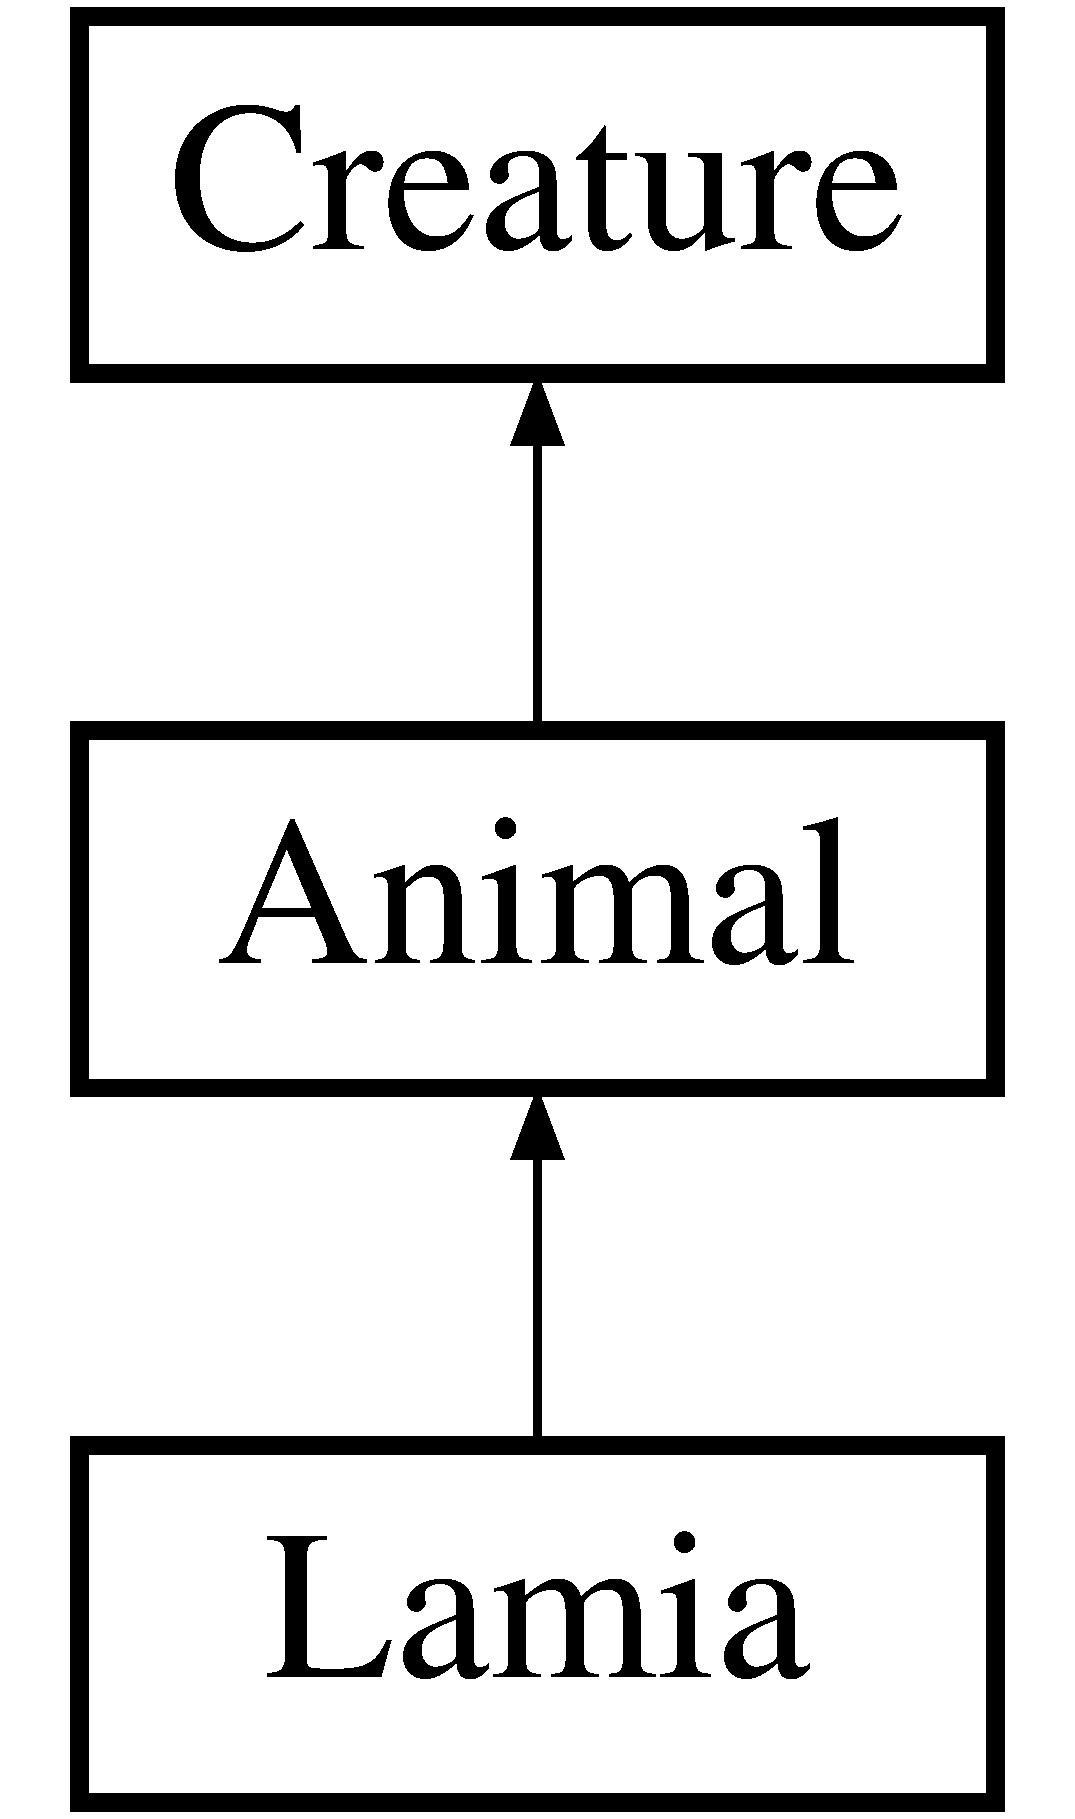
\includegraphics[height=3.000000cm]{class_lamia}
\end{center}
\end{figure}
\subsection*{Public Member Functions}
\begin{DoxyCompactItemize}
\item 
\hyperlink{class_lamia_a0fbc6a5d3b47d02f4455d24e6edf9000}{Lamia} (int=0, int=0, int=0, int=0)
\item 
void {\bfseries do\+Action} ()\hypertarget{class_lamia_a21663165aa075426083bf34fc6ff753d}{}\label{class_lamia_a21663165aa075426083bf34fc6ff753d}

\item 
char \hyperlink{class_lamia_a5bff769396d0bc31d03306ba1c190c39}{draw} ()
\end{DoxyCompactItemize}
\subsection*{Protected Member Functions}
\begin{DoxyCompactItemize}
\item 
void \hyperlink{class_lamia_a216ce1ca528e5bc3f35d882a4bd2cbc4}{move} ()
\end{DoxyCompactItemize}


\subsection{Constructor \& Destructor Documentation}
\index{Lamia@{Lamia}!Lamia@{Lamia}}
\index{Lamia@{Lamia}!Lamia@{Lamia}}
\subsubsection[{\texorpdfstring{Lamia(int=0, int=0, int=0, int=0)}{Lamia(int=0, int=0, int=0, int=0)}}]{\setlength{\rightskip}{0pt plus 5cm}Lamia\+::\+Lamia (
\begin{DoxyParamCaption}
\item[{int}]{r = {\ttfamily 0}, }
\item[{int}]{c = {\ttfamily 0}, }
\item[{int}]{x = {\ttfamily 0}, }
\item[{int}]{y = {\ttfamily 0}}
\end{DoxyParamCaption}
)}\hypertarget{class_lamia_a0fbc6a5d3b47d02f4455d24e6edf9000}{}\label{class_lamia_a0fbc6a5d3b47d02f4455d24e6edf9000}
Make \hyperlink{class_lamia}{Lamia} on postion (x,y) 
\begin{DoxyParams}{Parameters}
{\em x} & \\
\hline
{\em y} & \\
\hline
\end{DoxyParams}


\subsection{Member Function Documentation}
\index{Lamia@{Lamia}!draw@{draw}}
\index{draw@{draw}!Lamia@{Lamia}}
\subsubsection[{\texorpdfstring{draw()}{draw()}}]{\setlength{\rightskip}{0pt plus 5cm}char Lamia\+::draw (
\begin{DoxyParamCaption}
{}
\end{DoxyParamCaption}
)\hspace{0.3cm}{\ttfamily [virtual]}}\hypertarget{class_lamia_a5bff769396d0bc31d03306ba1c190c39}{}\label{class_lamia_a5bff769396d0bc31d03306ba1c190c39}
draw the \hyperlink{class_lamia}{Lamia} 

Implements \hyperlink{class_animal}{Animal}.

\index{Lamia@{Lamia}!move@{move}}
\index{move@{move}!Lamia@{Lamia}}
\subsubsection[{\texorpdfstring{move()}{move()}}]{\setlength{\rightskip}{0pt plus 5cm}void Lamia\+::move (
\begin{DoxyParamCaption}
{}
\end{DoxyParamCaption}
)\hspace{0.3cm}{\ttfamily [protected]}, {\ttfamily [virtual]}}\hypertarget{class_lamia_a216ce1ca528e5bc3f35d882a4bd2cbc4}{}\label{class_lamia_a216ce1ca528e5bc3f35d882a4bd2cbc4}
move the \hyperlink{class_lamia}{Lamia} 

Implements \hyperlink{class_animal}{Animal}.



The documentation for this class was generated from the following files\+:\begin{DoxyCompactItemize}
\item 
Lamia.\+h\item 
Lamia.\+cpp\end{DoxyCompactItemize}

\hypertarget{class_list}{}\section{List$<$ Type $>$ Class Template Reference}
\label{class_list}\index{List$<$ Type $>$@{List$<$ Type $>$}}
\subsection*{Public Member Functions}
\begin{DoxyCompactItemize}
\item 
\hyperlink{class_list_a87405d18413f3ec9e0b57ccfe39a5a1d}{List} ()
\item 
{\bfseries List} (Type data)\hypertarget{class_list_afbbfb958dda41678d9a138d3ad6a9b35}{}\label{class_list_afbbfb958dda41678d9a138d3ad6a9b35}

\item 
\hyperlink{class_list_ae52ebdc014f2709effb6a79917000b55}{List} (const \hyperlink{class_list}{List} \&L)
\item 
\hyperlink{class_list_a17633b3c9f5315c0888217947ab4bad1}{$\sim$\+List} ()
\item 
void \hyperlink{class_list_a8e1f80f098c0ef89dccb99d624f1d5ef}{Set\+Address\+List} (\hyperlink{class_element_list}{Element\+List}$<$ Type $>$ $\ast$L)
\item 
\hyperlink{class_element_list}{Element\+List}$<$ Type $>$ $\ast$ \hyperlink{class_list_a0f935df606117d95921002c4ec8da766}{Get\+Address\+List} ()
\item 
void \hyperlink{class_list_ae9238dae50d93e0276f9e721f32f5c10}{Insert\+Last} (Type data)
\item 
void \hyperlink{class_list_a00fce1708e871f4574c90942a3b71bb3}{Delete} (Type data)
\item 
bool \hyperlink{class_list_a4cc9e973d8289d39611b7750f01adbec}{is\+List\+Empty} ()
\end{DoxyCompactItemize}


\subsection{Constructor \& Destructor Documentation}
\index{List@{List}!List@{List}}
\index{List@{List}!List@{List}}
\subsubsection[{\texorpdfstring{List()}{List()}}]{\setlength{\rightskip}{0pt plus 5cm}template$<$class Type $>$ {\bf List}$<$ Type $>$\+::{\bf List} (
\begin{DoxyParamCaption}
{}
\end{DoxyParamCaption}
)}\hypertarget{class_list_a87405d18413f3ec9e0b57ccfe39a5a1d}{}\label{class_list_a87405d18413f3ec9e0b57ccfe39a5a1d}
Ctor of a generic \hyperlink{class_list}{List} \index{List@{List}!List@{List}}
\index{List@{List}!List@{List}}
\subsubsection[{\texorpdfstring{List(const List \&\+L)}{List(const List &L)}}]{\setlength{\rightskip}{0pt plus 5cm}template$<$class Type$>$ {\bf List}$<$ Type $>$\+::{\bf List} (
\begin{DoxyParamCaption}
\item[{const {\bf List}$<$ Type $>$ \&}]{L}
\end{DoxyParamCaption}
)}\hypertarget{class_list_ae52ebdc014f2709effb6a79917000b55}{}\label{class_list_ae52ebdc014f2709effb6a79917000b55}
Cctor of a generic \hyperlink{class_list}{List} \index{List@{List}!````~List@{$\sim$\+List}}
\index{````~List@{$\sim$\+List}!List@{List}}
\subsubsection[{\texorpdfstring{$\sim$\+List()}{~List()}}]{\setlength{\rightskip}{0pt plus 5cm}template$<$class Type $>$ {\bf List}$<$ Type $>$\+::$\sim${\bf List} (
\begin{DoxyParamCaption}
{}
\end{DoxyParamCaption}
)}\hypertarget{class_list_a17633b3c9f5315c0888217947ab4bad1}{}\label{class_list_a17633b3c9f5315c0888217947ab4bad1}
Dtor of a generic \hyperlink{class_list}{List} 

\subsection{Member Function Documentation}
\index{List@{List}!Delete@{Delete}}
\index{Delete@{Delete}!List@{List}}
\subsubsection[{\texorpdfstring{Delete(\+Type data)}{Delete(Type data)}}]{\setlength{\rightskip}{0pt plus 5cm}template$<$class Type$>$ void {\bf List}$<$ Type $>$\+::Delete (
\begin{DoxyParamCaption}
\item[{Type}]{data}
\end{DoxyParamCaption}
)}\hypertarget{class_list_a00fce1708e871f4574c90942a3b71bb3}{}\label{class_list_a00fce1708e871f4574c90942a3b71bb3}
Delete an data from the list 
\begin{DoxyParams}{Parameters}
{\em data} & \\
\hline
\end{DoxyParams}
\index{List@{List}!Get\+Address\+List@{Get\+Address\+List}}
\index{Get\+Address\+List@{Get\+Address\+List}!List@{List}}
\subsubsection[{\texorpdfstring{Get\+Address\+List()}{GetAddressList()}}]{\setlength{\rightskip}{0pt plus 5cm}template$<$class Type $>$ {\bf Element\+List}$<$ Type $>$ $\ast$ {\bf List}$<$ Type $>$\+::Get\+Address\+List (
\begin{DoxyParamCaption}
{}
\end{DoxyParamCaption}
)}\hypertarget{class_list_a0f935df606117d95921002c4ec8da766}{}\label{class_list_a0f935df606117d95921002c4ec8da766}
Get the Adress of \hyperlink{class_list}{List} \index{List@{List}!Insert\+Last@{Insert\+Last}}
\index{Insert\+Last@{Insert\+Last}!List@{List}}
\subsubsection[{\texorpdfstring{Insert\+Last(\+Type data)}{InsertLast(Type data)}}]{\setlength{\rightskip}{0pt plus 5cm}template$<$class Type$>$ void {\bf List}$<$ Type $>$\+::Insert\+Last (
\begin{DoxyParamCaption}
\item[{Type}]{data}
\end{DoxyParamCaption}
)}\hypertarget{class_list_ae9238dae50d93e0276f9e721f32f5c10}{}\label{class_list_ae9238dae50d93e0276f9e721f32f5c10}
Insert a data to last of the list 
\begin{DoxyParams}{Parameters}
{\em data} & \\
\hline
\end{DoxyParams}
\index{List@{List}!is\+List\+Empty@{is\+List\+Empty}}
\index{is\+List\+Empty@{is\+List\+Empty}!List@{List}}
\subsubsection[{\texorpdfstring{is\+List\+Empty()}{isListEmpty()}}]{\setlength{\rightskip}{0pt plus 5cm}template$<$class Type $>$ bool {\bf List}$<$ Type $>$\+::is\+List\+Empty (
\begin{DoxyParamCaption}
{}
\end{DoxyParamCaption}
)}\hypertarget{class_list_a4cc9e973d8289d39611b7750f01adbec}{}\label{class_list_a4cc9e973d8289d39611b7750f01adbec}
Return 1 if \hyperlink{class_list}{List} empty, 0 otherwise \index{List@{List}!Set\+Address\+List@{Set\+Address\+List}}
\index{Set\+Address\+List@{Set\+Address\+List}!List@{List}}
\subsubsection[{\texorpdfstring{Set\+Address\+List(\+Element\+List$<$ Type $>$ $\ast$\+L)}{SetAddressList(ElementList< Type > *L)}}]{\setlength{\rightskip}{0pt plus 5cm}template$<$class Type$>$ void {\bf List}$<$ Type $>$\+::Set\+Address\+List (
\begin{DoxyParamCaption}
\item[{{\bf Element\+List}$<$ Type $>$ $\ast$}]{L}
\end{DoxyParamCaption}
)}\hypertarget{class_list_a8e1f80f098c0ef89dccb99d624f1d5ef}{}\label{class_list_a8e1f80f098c0ef89dccb99d624f1d5ef}
Set the Adress of \hyperlink{class_list}{List} 
\begin{DoxyParams}{Parameters}
{\em L} & \\
\hline
\end{DoxyParams}


The documentation for this class was generated from the following files\+:\begin{DoxyCompactItemize}
\item 
list.\+h\item 
list.\+cpp\end{DoxyCompactItemize}

\hypertarget{structmove_direction}{}\section{move\+Direction Struct Reference}
\label{structmove_direction}\index{move\+Direction@{move\+Direction}}
\subsection*{Public Attributes}
\begin{DoxyCompactItemize}
\item 
int {\bfseries deltax}\hypertarget{structmove_direction_a3178a4b35b2c721742ba680a99ee526c}{}\label{structmove_direction_a3178a4b35b2c721742ba680a99ee526c}

\item 
int {\bfseries deltay}\hypertarget{structmove_direction_a67c6f8ff956f588e8a534cecbbf18248}{}\label{structmove_direction_a67c6f8ff956f588e8a534cecbbf18248}

\end{DoxyCompactItemize}


The documentation for this struct was generated from the following file\+:\begin{DoxyCompactItemize}
\item 
Animal.\+h\end{DoxyCompactItemize}

\hypertarget{class_plant}{}\section{Plant Class Reference}
\label{class_plant}\index{Plant@{Plant}}
Inheritance diagram for Plant\+:\begin{figure}[H]
\begin{center}
\leavevmode
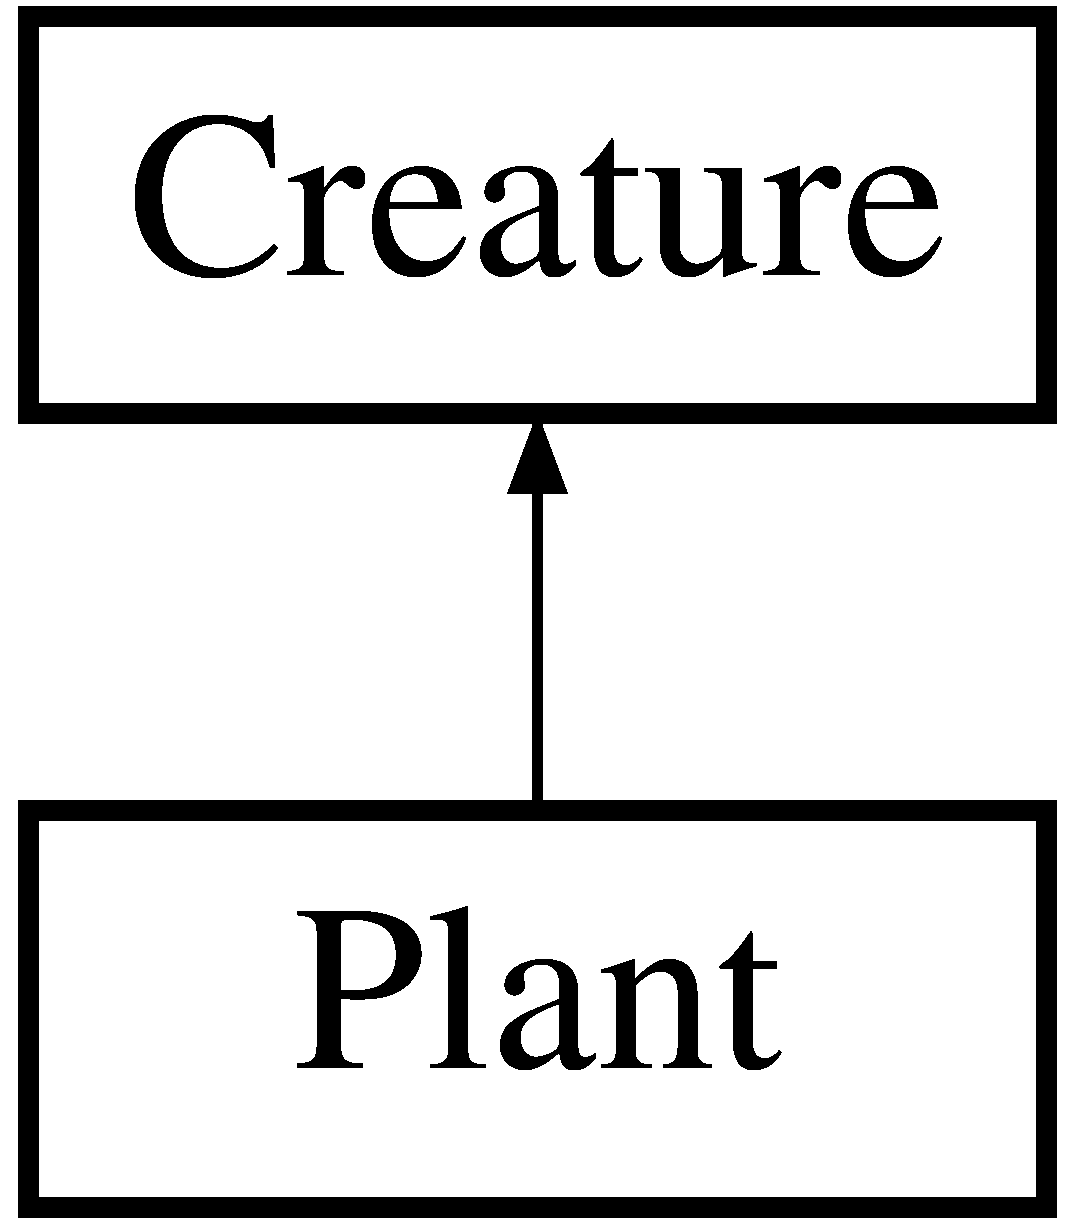
\includegraphics[height=2.000000cm]{class_plant}
\end{center}
\end{figure}
\subsection*{Public Member Functions}
\begin{DoxyCompactItemize}
\item 
\hyperlink{class_plant_a3b0ca01a599b8a7348afe2cef1ad8613}{Plant} (int=0, int=0)
\item 
char \hyperlink{class_plant_a6fb833eaf05ea95be02cef14412830cc}{draw} ()
\item 
void {\bfseries do\+Action} ()\hypertarget{class_plant_abbb1927a780865746a611127cc26feb9}{}\label{class_plant_abbb1927a780865746a611127cc26feb9}

\end{DoxyCompactItemize}


\subsection{Constructor \& Destructor Documentation}
\index{Plant@{Plant}!Plant@{Plant}}
\index{Plant@{Plant}!Plant@{Plant}}
\subsubsection[{\texorpdfstring{Plant(int=0, int=0)}{Plant(int=0, int=0)}}]{\setlength{\rightskip}{0pt plus 5cm}Plant\+::\+Plant (
\begin{DoxyParamCaption}
\item[{int}]{\+\_\+r = {\ttfamily 0}, }
\item[{int}]{\+\_\+c = {\ttfamily 0}}
\end{DoxyParamCaption}
)}\hypertarget{class_plant_a3b0ca01a599b8a7348afe2cef1ad8613}{}\label{class_plant_a3b0ca01a599b8a7348afe2cef1ad8613}
Make \hyperlink{class_plant}{Plant} on postion (x,y) 
\begin{DoxyParams}{Parameters}
{\em data} & \\
\hline
\end{DoxyParams}


\subsection{Member Function Documentation}
\index{Plant@{Plant}!draw@{draw}}
\index{draw@{draw}!Plant@{Plant}}
\subsubsection[{\texorpdfstring{draw()}{draw()}}]{\setlength{\rightskip}{0pt plus 5cm}char Plant\+::draw (
\begin{DoxyParamCaption}
{}
\end{DoxyParamCaption}
)\hspace{0.3cm}{\ttfamily [virtual]}}\hypertarget{class_plant_a6fb833eaf05ea95be02cef14412830cc}{}\label{class_plant_a6fb833eaf05ea95be02cef14412830cc}
draw the \hyperlink{class_plant}{Plant} 
\begin{DoxyParams}{Parameters}
{\em data} & \\
\hline
\end{DoxyParams}


Implements \hyperlink{class_creature}{Creature}.



The documentation for this class was generated from the following files\+:\begin{DoxyCompactItemize}
\item 
Plant.\+h\item 
Plant.\+cpp\end{DoxyCompactItemize}

\hypertarget{class_universe}{}\section{Universe Class Reference}
\label{class_universe}\index{Universe@{Universe}}
Inheritance diagram for Universe\+:\begin{figure}[H]
\begin{center}
\leavevmode
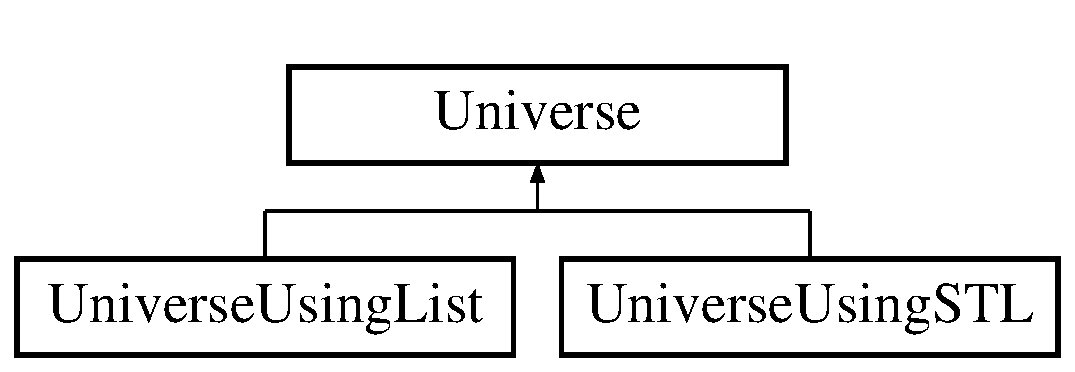
\includegraphics[height=2.000000cm]{class_universe}
\end{center}
\end{figure}
\subsection*{Public Member Functions}
\begin{DoxyCompactItemize}
\item 
{\bfseries Universe} (int, int)\hypertarget{class_universe_ad3f8dfc7f0c2e14d08779fc84a8d893a}{}\label{class_universe_ad3f8dfc7f0c2e14d08779fc84a8d893a}

\item 
int {\bfseries get\+Amount\+Of\+Rows} ()\hypertarget{class_universe_a8f219d93acf88902438497356fb4b79d}{}\label{class_universe_a8f219d93acf88902438497356fb4b79d}

\item 
int {\bfseries get\+Amount\+Of\+Columns} ()\hypertarget{class_universe_a5b0a0f6b1927e223b0a18f2474a05711}{}\label{class_universe_a5b0a0f6b1927e223b0a18f2474a05711}

\item 
void {\bfseries set\+Amount\+Of\+Rows} (int)\hypertarget{class_universe_af0124aca57a7ff286132e8525bd1c378}{}\label{class_universe_af0124aca57a7ff286132e8525bd1c378}

\item 
void {\bfseries set\+Amount\+Of\+Columns} (int)\hypertarget{class_universe_a9597c59c4bf80e17c852596acf25dfc4}{}\label{class_universe_a9597c59c4bf80e17c852596acf25dfc4}

\item 
virtual void {\bfseries kill\+Creature} (\hyperlink{class_creature}{Creature} $\ast$)=0\hypertarget{class_universe_ae92953c55e994fd3db8ac022ef69c227}{}\label{class_universe_ae92953c55e994fd3db8ac022ef69c227}

\item 
virtual void {\bfseries add\+Creature} (\hyperlink{class_creature}{Creature} $\ast$)=0\hypertarget{class_universe_a882e14be433281816c58b9ccfb8d4d01}{}\label{class_universe_a882e14be433281816c58b9ccfb8d4d01}

\item 
virtual void {\bfseries add\+Random\+Creature} (int)=0\hypertarget{class_universe_a7289af8da66eed7c88763342c5689efb}{}\label{class_universe_a7289af8da66eed7c88763342c5689efb}

\item 
virtual int {\bfseries is\+World\+Empty} ()=0\hypertarget{class_universe_a090dce863386ed5cdba01d440de1edfd}{}\label{class_universe_a090dce863386ed5cdba01d440de1edfd}

\item 
virtual void {\bfseries check\+For\+Collisions} ()=0\hypertarget{class_universe_aaefe829c75ee2290de431e16065dde83}{}\label{class_universe_aaefe829c75ee2290de431e16065dde83}

\item 
virtual void {\bfseries create\+Threads\+For\+Creatures} ()=0\hypertarget{class_universe_ab7d79c7d4f6c76f9f15ba1aec1c81c9f}{}\label{class_universe_ab7d79c7d4f6c76f9f15ba1aec1c81c9f}

\item 
virtual void {\bfseries move\+All\+Creatures\+Once} ()=0\hypertarget{class_universe_af6fafeecd9df7c0c2b83760cef4eced3}{}\label{class_universe_af6fafeecd9df7c0c2b83760cef4eced3}

\item 
virtual void {\bfseries print} (ostream \&)=0\hypertarget{class_universe_a646c85dce1a89e8da9b7f8c7c71cb2e3}{}\label{class_universe_a646c85dce1a89e8da9b7f8c7c71cb2e3}

\end{DoxyCompactItemize}


The documentation for this class was generated from the following files\+:\begin{DoxyCompactItemize}
\item 
Universe.\+h\item 
Universe.\+cpp\end{DoxyCompactItemize}

\hypertarget{class_universe_using_list}{}\section{Universe\+Using\+List Class Reference}
\label{class_universe_using_list}\index{Universe\+Using\+List@{Universe\+Using\+List}}
Inheritance diagram for Universe\+Using\+List\+:\begin{figure}[H]
\begin{center}
\leavevmode
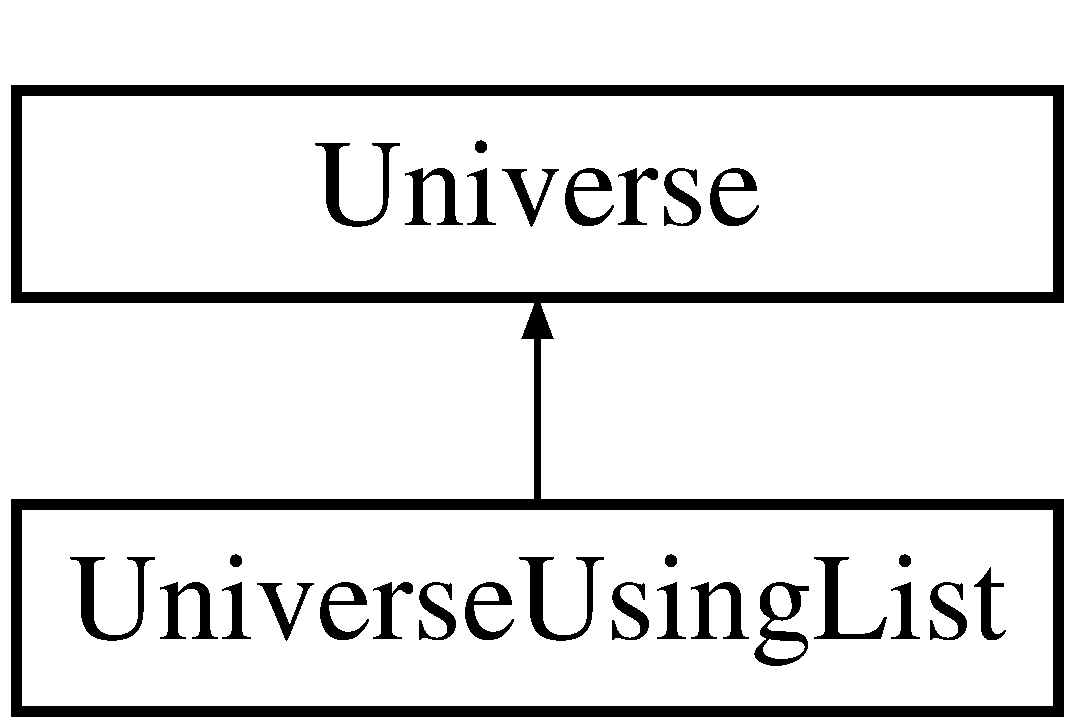
\includegraphics[height=2.000000cm]{class_universe_using_list}
\end{center}
\end{figure}
\subsection*{Public Member Functions}
\begin{DoxyCompactItemize}
\item 
{\bfseries Universe\+Using\+List} (int, int)\hypertarget{class_universe_using_list_a690190032d86eadad922b33166d6d11a}{}\label{class_universe_using_list_a690190032d86eadad922b33166d6d11a}

\item 
void {\bfseries kill\+Creature} (\hyperlink{class_creature}{Creature} $\ast$C)\hypertarget{class_universe_using_list_ad5ae1ddeb1ea11111e506373de5364d8}{}\label{class_universe_using_list_ad5ae1ddeb1ea11111e506373de5364d8}

\item 
void {\bfseries add\+Creature} (\hyperlink{class_creature}{Creature} $\ast$C)\hypertarget{class_universe_using_list_a936d1a839b5cd80f9715c7f2e2daf1da}{}\label{class_universe_using_list_a936d1a839b5cd80f9715c7f2e2daf1da}

\item 
void {\bfseries add\+Random\+Creature} (int amount)\hypertarget{class_universe_using_list_a77570a26fbc9bc108c94ea815ce4bb67}{}\label{class_universe_using_list_a77570a26fbc9bc108c94ea815ce4bb67}

\item 
void {\bfseries print} (ostream \&)\hypertarget{class_universe_using_list_a9cbe5a6b7497005e60131907a3aa8120}{}\label{class_universe_using_list_a9cbe5a6b7497005e60131907a3aa8120}

\end{DoxyCompactItemize}


The documentation for this class was generated from the following files\+:\begin{DoxyCompactItemize}
\item 
Universe\+Using\+List.\+h\item 
Universe\+Using\+List.\+cpp\end{DoxyCompactItemize}

%--- End generated contents ---

% Index
\backmatter
\newpage
\phantomsection
\clearemptydoublepage
\addcontentsline{toc}{chapter}{Index}
\printindex

\end{document}
